\documentclass{beamer}
\usetheme[sectionpage=progressbar, subsectionpage=progressbar, numbering=fraction, progressbar=foot, block=fill, background=light]{metropolis}
\usepackage{appendixnumberbeamer}
\usepackage{textpos}
\usepackage{booktabs}
\usepackage[scale=2]{ccicons}

\usepackage{pgfplots}
\usepgfplotslibrary{dateplot}
\usetikzlibrary{backgrounds}
\usepackage{xspace}
\newcommand{\themename}{\textbf{\textsc{metropolis}}\xspace}
\title{Attention based models in End-to-End ASR}
\subtitle{Exploration of Attention in ESPNET toolkit}
\date{\today}
\author{Shreekantha Nadig}
\institute{International Institute of Information Technology - Bangalore}
%\titlegraphic{\hfill\includegraphics[height=1.5cm]{logo.pdf}}

\usepackage{tikz}
\usetikzlibrary{shapes,shadows,arrows,patterns, matrix}

\tikzstyle{line} = [draw, -latex']
\tikzstyle{round} = [draw, circle, fill=black!30, minimum size=4em, node distance=4em, font=\fontsize{30}{10}\selectfont]
\tikzstyle{mlp_enc} = [rectangle, draw, fill=red!50, text width=2cm, minimum height=5em, text centered, node distance=10em, font=\fontsize{20}{10}\selectfont]
\tikzstyle{mlp_att} = [rectangle, draw, fill=green!50, text width=2cm, minimum height=5em, text centered, node distance=10em, font=\fontsize{20}{10}\selectfont]
\tikzstyle{mlp_dec} = [rectangle, draw, fill=blue!50, text width=2cm, minimum height=5em, text centered, node distance=10em, font=\fontsize{20}{10}\selectfont]
\tikzstyle{enc_h} = [rectangle, draw,  pattern=horizontal lines, pattern color=red!60, text width=1cm, minimum height=10em, minimum width=3em, text centered, node distance=10em, font=\fontsize{25}{10}\selectfont]
\tikzstyle{atts} = [rectangle, draw,  pattern=horizontal lines, pattern color=green!70, text width=1cm, minimum height=10em, minimum width=3em, text centered, node distance=10em, font=\fontsize{20}{10}\selectfont]
\tikzstyle{dec_z} = [rectangle, draw,  pattern=horizontal lines, pattern color=blue!60, text width=1cm, minimum height=10em, minimum width=3em, text centered, node distance=10em, font=\fontsize{20}{10}\selectfont]
\tikzstyle{cnn} = [rectangle, draw,  pattern=crosshatch, pattern color=red!50!blue!50, text width=2cm, minimum height=5em, text centered, node distance=10em, font=\fontsize{20}{10}\selectfont]
\tikzstyle{box} = [rectangle, draw,  fill=blue!20, text width=3cm, minimum height=5em, minimum width=3em, text centered, node distance=10em, font=\fontsize{20}{10}\selectfont]

\begin{document}
	\addtobeamertemplate{frametitle}{}{%
		\begin{textblock*}{100mm}(.97\textwidth,-1cm)
			{
\includegraphics[width=2.5em]{iiitb_logo.png}}
		\end{textblock*}}

%\maketitle

\begin{frame}[fragile]{Scaled Dot product}
\begin{center}
	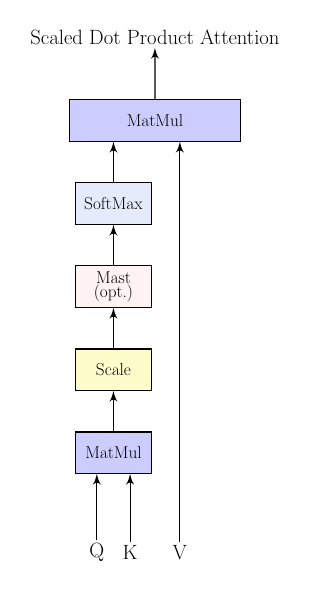
\begin{tikzpicture}[scale=0.3, every node/.style={transform shape, font=\fontsize{40}{40}\selectfont}]
	
	\node [box] (mm1) {MatMul};
	\node [box, above of = mm1, fill=yellow!20] (scale1) {Scale};
	\node [box, above of = scale1, fill=pink!20] (mask) {Mast (opt.)};
	\node [box, above of = mask, fill=green!20!blue!10] (sm) {SoftMax};
	\node [box, above of = sm, xshift = 5em, text width = 20em] (mm2) {MatMul};
	\node [below of=mm1, node distance = 12em, xshift = -2em] (q) {Q};
	\node [below of=mm1, node distance = 12em, xshift = 2em] (k) {K};
	\node [below of=mm1, node distance = 12em, xshift = 8em] (v) {V};
	
	\path [line] (k.north) -- (k.north |- mm1.south);
	\path [line] (q.north) -- (q.north |- mm1.south);
	\path [line] (v.north) -- (v.north |- mm2.south);
	
	\path [line] (mm1.north) to (scale1.south);
	\path [line] (scale1.north) to (mask.south);
	\path [line] (mask.north) to (sm.south);
	\path [line] (sm.north) -- (sm.north |- mm2.south);
	
	\node [above of = mm2, node distance = 10em] (e) {Scaled Dot Product Attention};
	\path [line] (mm2.north) to (e.south);
	\end{tikzpicture}
\end{center}
\end{frame}


\begin{frame}[fragile]{Multi-Head Attention}
\begin{center}
	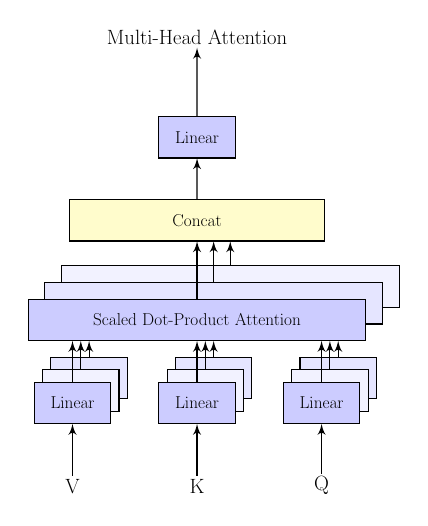
\begin{tikzpicture}[scale=0.3, every node/.style={transform shape, font=\fontsize{40}{40}\selectfont}]
	
	\node [box] (lin1) {Linear};
	\node [box, right of=lin1, node distance = 15em] (lin2) {Linear};
	\node [box, right of=lin2, node distance = 15em] (lin3) {Linear};
	
	\node [box, above of = lin2, text width = 40em] (sd1) {Scaled Dot-Product Attention};
	
	\begin{scope}[on background layer]
	\node [box, above of = lin1, node distance = 3em, fill=blue!10, xshift=2em, fill=blue!10] (lin22)
	{};
	\node [box, above of = lin1, node distance = 1.5em, fill=blue!10, xshift=1em, fill=blue!5] (lin21)
	{};
	
	\node [box, above of = lin2, node distance = 3em, fill=blue!10, xshift=2em, fill=blue!10] (lin32)
	{};
	\node [box, above of = lin2, node distance = 1.5em, fill=blue!10, xshift=1em, fill=blue!5] (lin31)
	{};
	
	\node [box, above of = lin3, node distance = 3em, fill=blue!10, xshift=2em, fill=blue!10] (lin42)
	{};
	\node [box, above of = lin3, node distance = 1.5em, fill=blue!10, xshift=1em, fill=blue!5] (lin41)
	{};
	
	\node [box, above of = sd1, text width = 40em, node distance = 4em, xshift = 4em, fill=blue!5] (sd3) {};
	\node [box, above of = sd1, text width = 40em, node distance = 2em, xshift = 2em, fill=blue!10] (sd2) {};
	\end{scope}
	
	\path [line] (lin1.north) -- (lin1.north |- sd1.south);
	\path [line] (lin2.north) -- (lin2.north |- sd1.south);
	\path [line] (lin3.north) -- (lin3.north |- sd1.south);
	
	\path [line] (lin22.north) -- (lin22.north |- sd1.south);
	\path [line] (lin32.north) -- (lin32.north |- sd1.south);
	\path [line] (lin42.north) -- (lin42.north |- sd1.south);
	
	\path [line] (lin21.north) -- (lin21.north |- sd1.south);
	\path [line] (lin31.north) -- (lin31.north |- sd1.south);
	\path [line] (lin41.north) -- (lin41.north |- sd1.south);
	
	\node [box, above of = sd1, node distance = 12em, fill=yellow!20, text width = 30em] (concat) {Concat};
	\node [box, above of = concat] (linear) {Linear};
	
	\path [line] (sd1.north) -- (sd1.north |- concat.south);
	\path [line] (sd2.north) -- (sd2.north |- concat.south);
	\path [line] (sd3.north) -- (sd3.north |- concat.south);
	\path [line] (concat.north) to (linear.south);
	
	\node [above of = linear, node distance = 12em] (mh) {Multi-Head Attention};
	\path [line] (linear.north) to (mh.south);
	
	\node [below of=lin1, node distance = 10em] (V) {V};
	\node [below of=lin2, node distance = 10em] (K) {K};
	\node [below of=lin3, node distance = 10em] (Q) {Q};
	
	\path [line] (V.north) -- (V.north |- lin1.south);
	\path [line] (K.north) -- (K.north |- lin2.south);
	\path [line] (Q.north) -- (Q.north |- lin3.south);
	
	\end{tikzpicture}
\end{center}
\end{frame}


\begin{frame}[fragile]{The Transformer - model architecture}
\begin{center}

	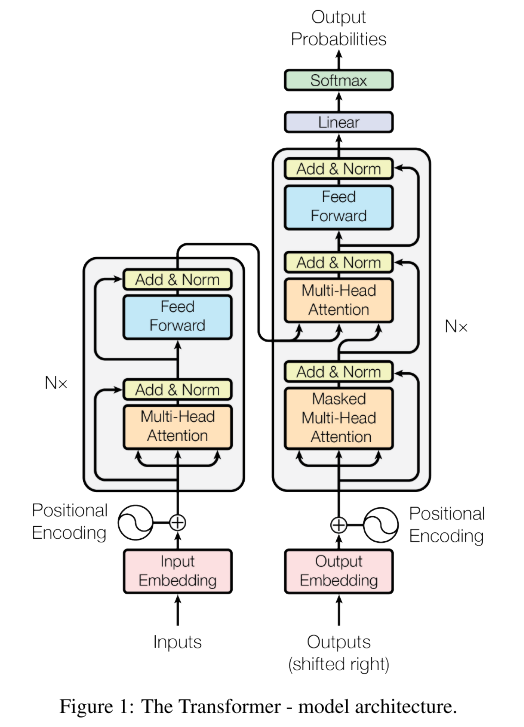
\includegraphics[width=\textwidth,height=\textheight,keepaspectratio]{mh_att.png}

\end{center}
\end{frame}


\begin{frame}[fragile]{Positional Encoding - Example}
\begin{center}
	
	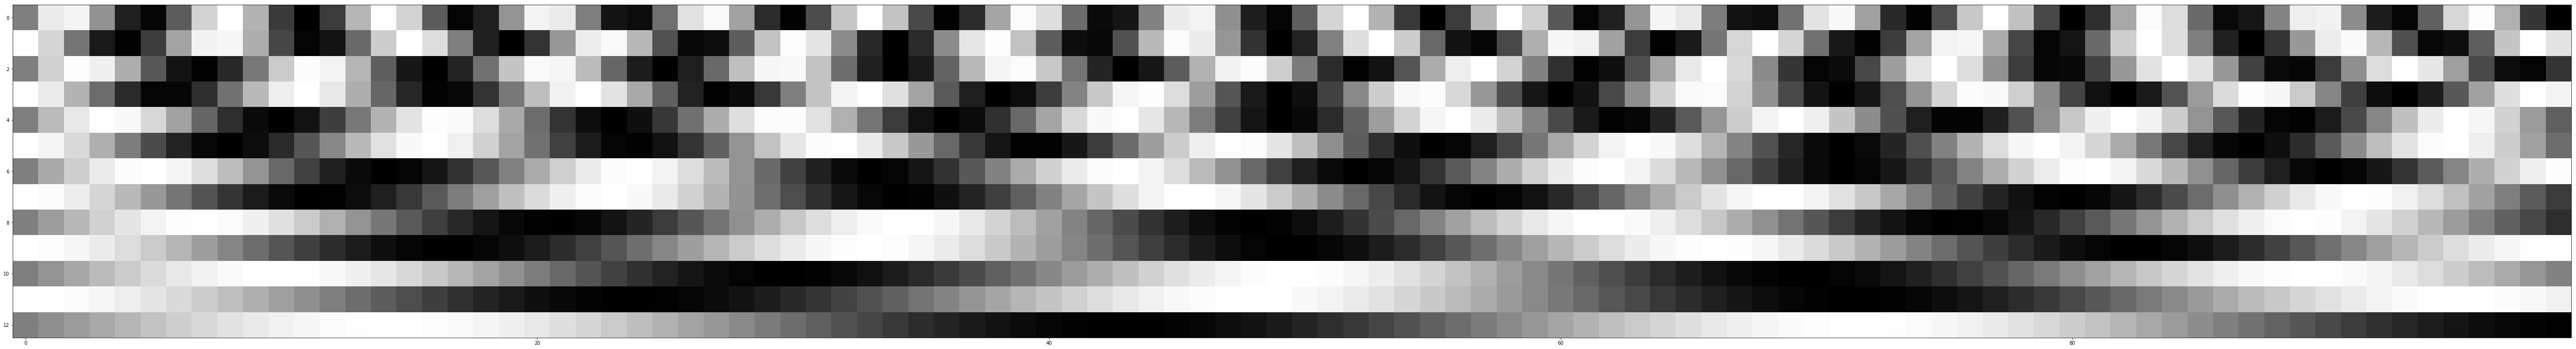
\includegraphics[width=\textwidth,height=\textheight,keepaspectratio]{pos_enc.png}
	$$PE_{(pos, 2_{i})} = sin(pos/1000^{2i/d_{model}})$$
	$$PE_{(pos, 2_{i+1})} = cos(pos/1000^{2i/d_{model}})$$
\end{center}
\end{frame}


\end{document}